%%===========================================================%%
%%                                                           %%
%%              DEAD MATERIAL IN FRONT OF TPC                %%
%%                                                           %%
%%===========================================================%%


\newcommand{\itemm}{\item\hspace*{-5pt}.\hspace*{-1pt}~}

\chapter{Dead material in front of TPC}\label{chap:deadMaterial}

Particle detected and reconstructed in the TPC must first pass through the detector material standing in between the accelerator vacuum and TPC gas. This affects track reconstruction efficiency, as the particle may interact with that material - in worst case inelastically, and induce secondary particles thus lower reconstruction efficiency. Accuracy of modeling of the detector material in the STAR simulation, especially in run 15 with the HFT installed, influences systematic error e.g. on the TPC track reconstruction efficiency. In this section the density of secondary vertices is compared between the data and embedded MC. The density of secondary vertices is directly propotional to the amount of the material in given volume, hence any discrepancy between secondary vertex distribution in the data and MC can be a hint for innacuracies of the STAR simulation which should be accordingly covered by the systematic uncertainties. It should be stressed that this analysis is not aimed to tune the material budget in the STAR simulation, as there are much better data for this than high-luminosity proton-proton collisions from run 15. The aim of presented study is to obtain reasonable estimate of the component of systematic uncertainty of the TPC track reconstruction effciency related to the error on the amount and distribution of simulated material.

%---------------------------
\begin{figure}[b!]\vspace{-10pt}
\centering
\parbox{0.4725\textwidth}{
  \centering
  \begin{subfigure}[b]{\linewidth}
                \subcaptionbox{\label{fig:multDataVsMC}}{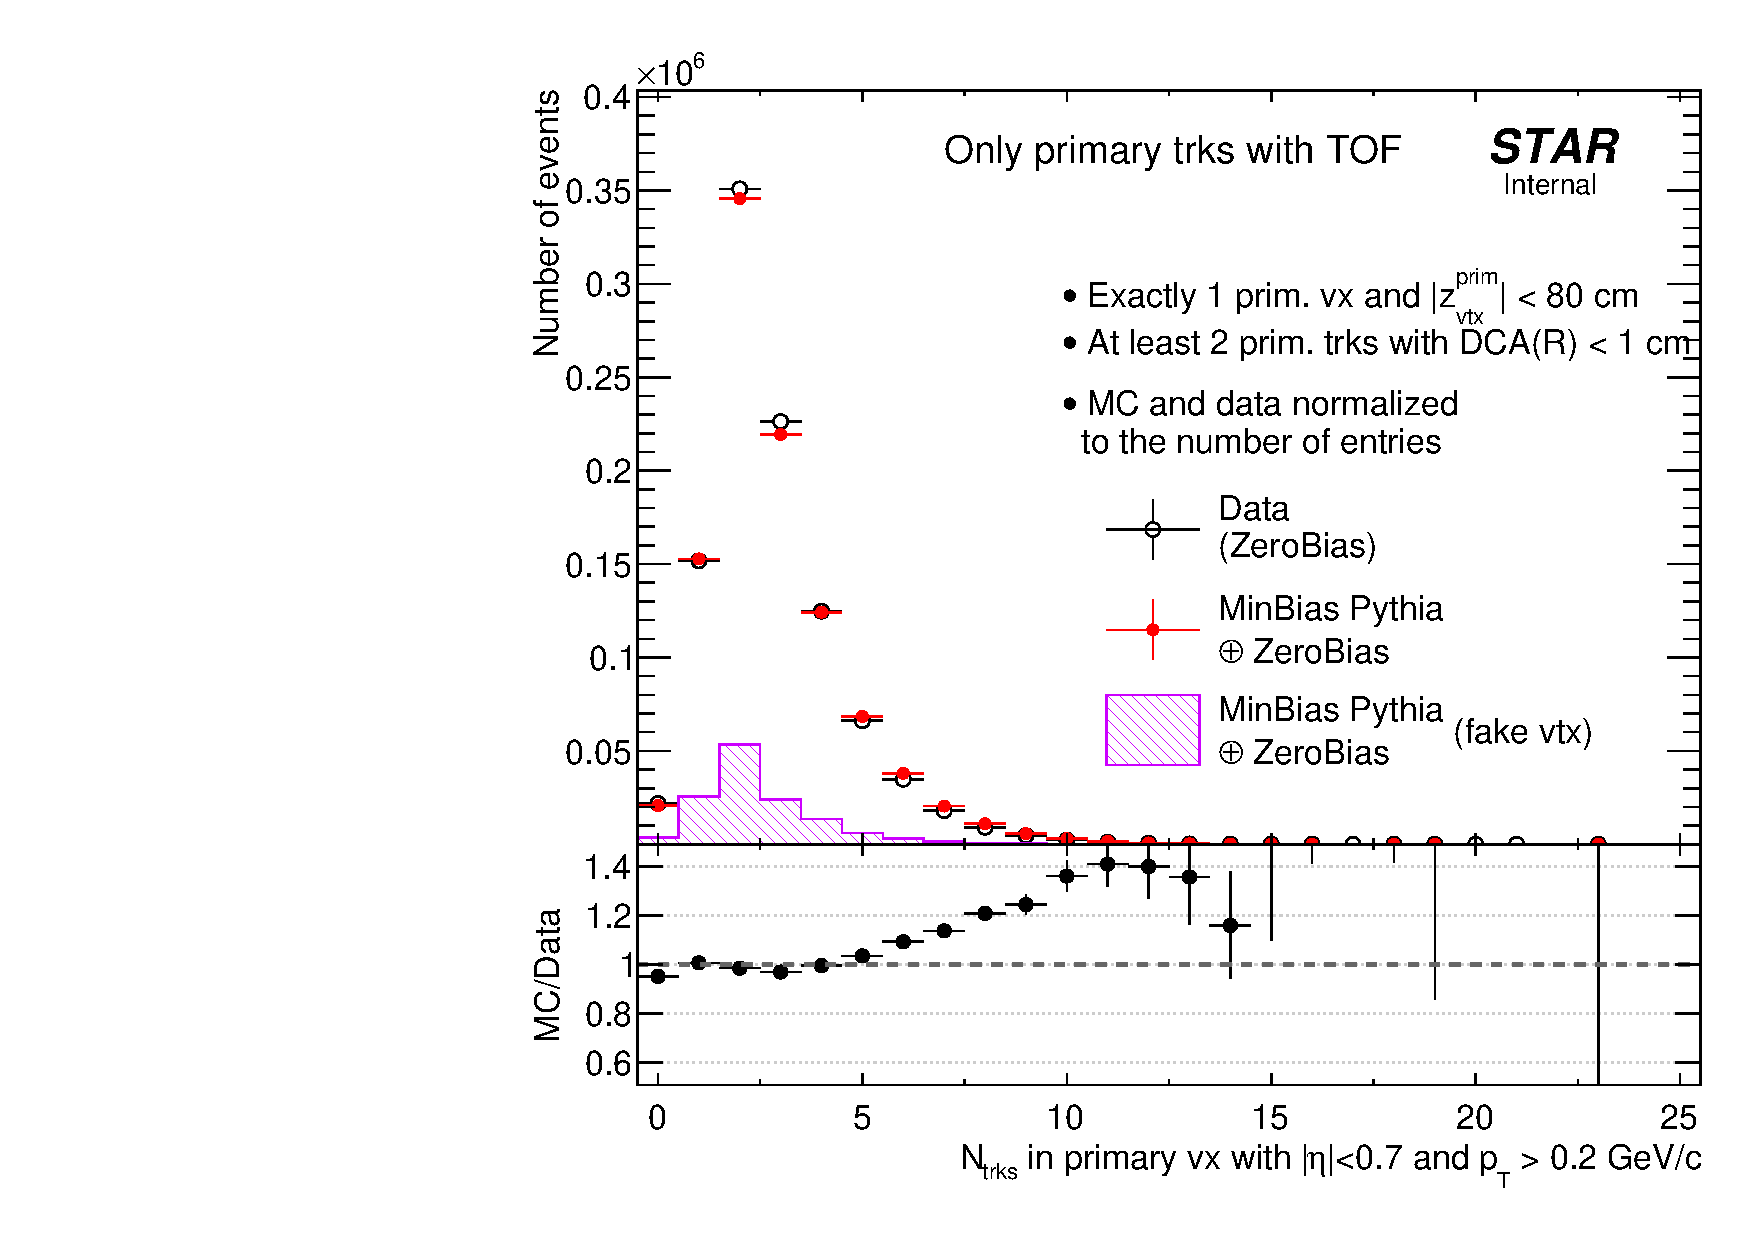
\includegraphics[width=\linewidth]{graphics/deadMaterial/NTracksPrimary_SelectedEvents_EtaPtCut_DataVsMC.pdf}}
  \end{subfigure}\\
  \begin{subfigure}[b]{\linewidth}\addtocounter{subfigure}{1}
                \subcaptionbox{\label{fig:etaDataVsMC}}{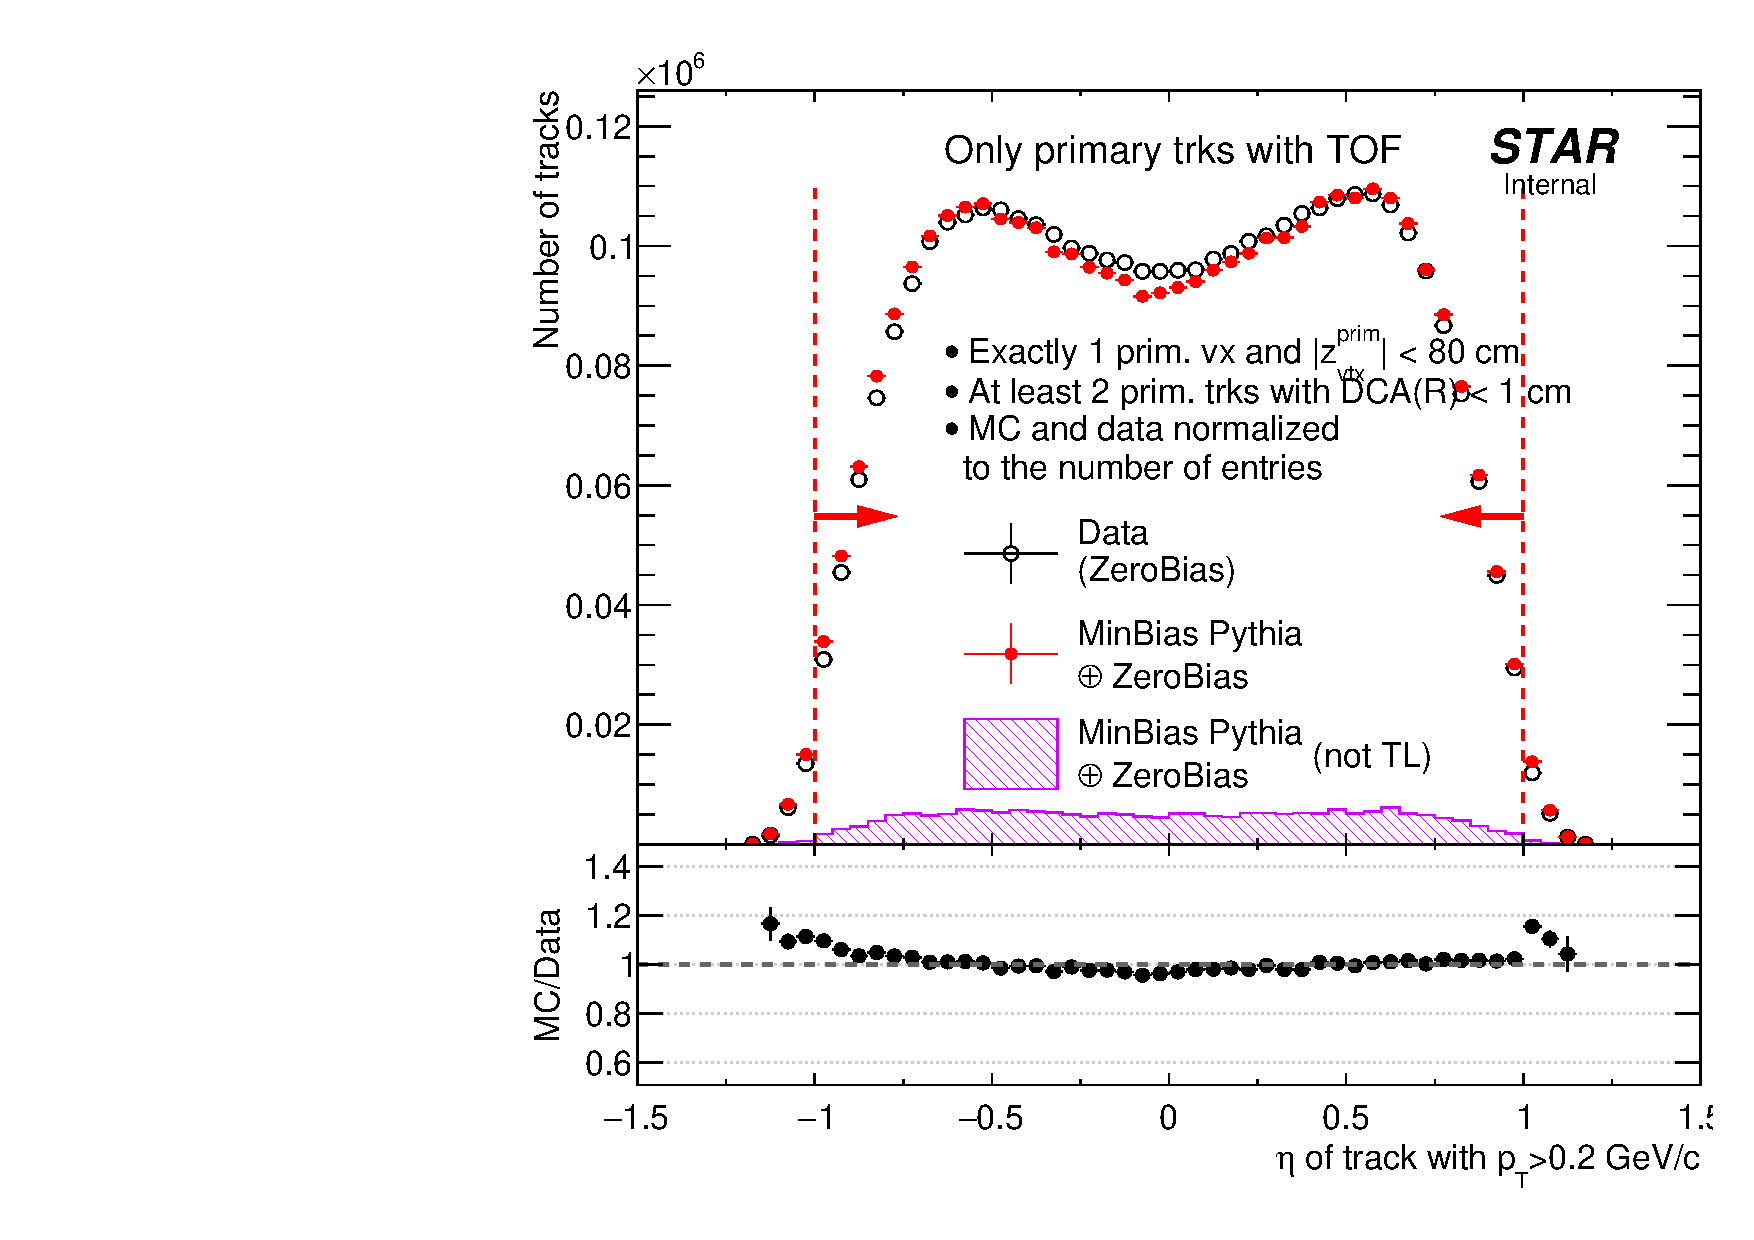
\includegraphics[width=\linewidth]{graphics/deadMaterial/TrackEtaPrimary_SelectedEvents_DataVsMC.pdf}}
  \end{subfigure}
}%
\quad\quad%
\parbox{0.4725\textwidth}{
  \centering
  \begin{subfigure}[b]{\linewidth}\addtocounter{subfigure}{-2}
                \subcaptionbox{\label{fig:ptDataVsMC}}{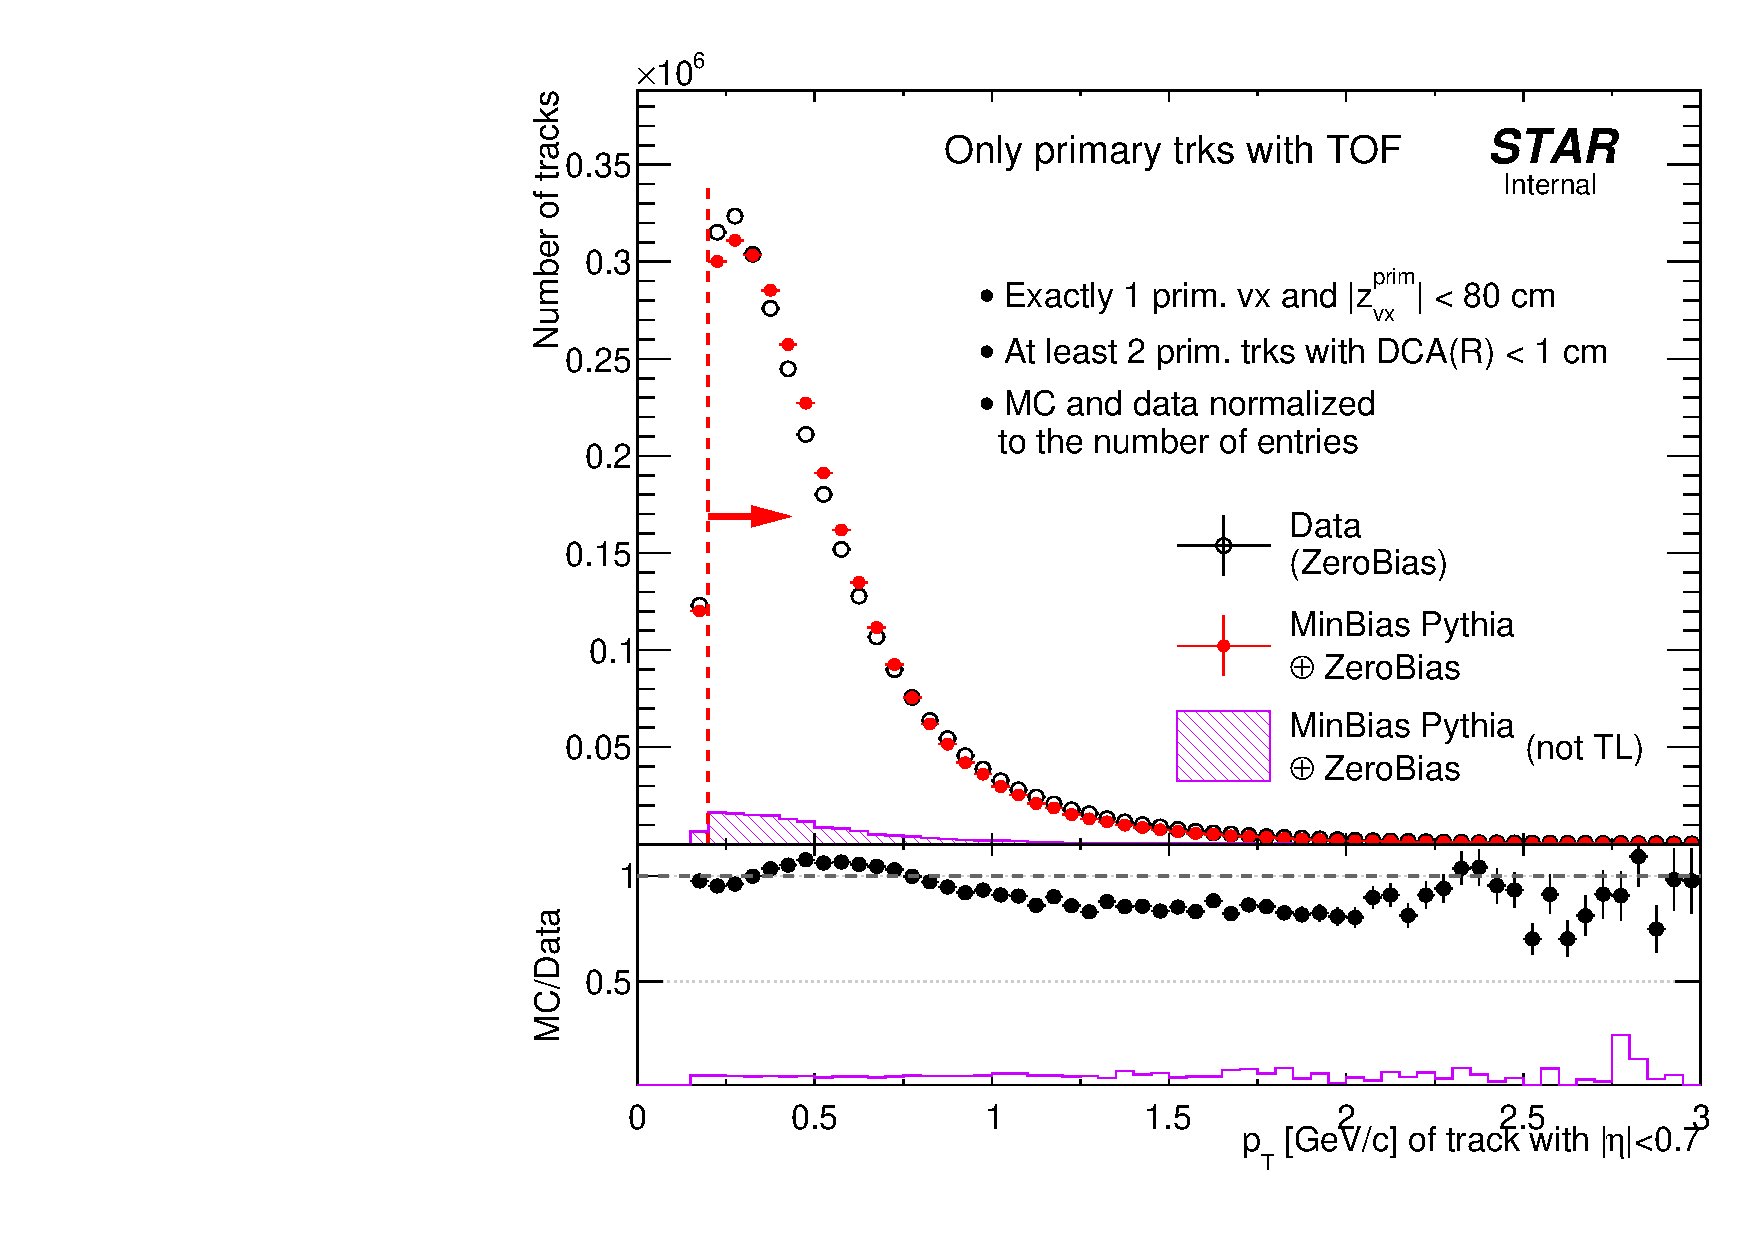
\includegraphics[width=\linewidth]{graphics/deadMaterial/TrackPtPrimary_SelectedEvents_DataVsMC.pdf}}
  \end{subfigure}\\
  \begin{minipage}[t][1.042\linewidth][t]{\linewidth}\vspace{10pt}
    \caption[Comparison of primary track multiplicity, $p_{T}$ and $\eta$ distribution in zero-bias data and embedded MC (minimum-bias).]%
    {Comparison of primary track multiplicity~(\ref{fig:multDataVsMC}), $p_{T}$~(\ref{fig:ptDataVsMC}) and $\eta$~(\ref{fig:etaDataVsMC}) distribution in zero-bias data and minimum-bias MC embedded into zero-bias triggers. In all subfigures MC histogram is normalized to have the same integral as the data histogram. Violet hashed histogram in Fig.~\ref{fig:multDataVsMC} represents the fake vertices defined as vertices of which less than a half of constituent tracks is matched to true-level particles. Violet hashed histogram in Fig.~\ref{fig:ptDataVsMC} and~\ref{fig:etaDataVsMC} represents tracks not matched to true-level particles. Bottom pads in each figure show the ratio between MC and data as black points, and the ratio between fake (violet histogram) and all MC entries (red points) as a violet line. Red dashed lines and arrows indicate range of tracks required in selection of events for the secondary vertex analysis.}\label{fig:deadMatDataVsMC}
  \end{minipage}
}\vspace{-20pt}%
\end{figure}
%---------------------------

Analysis of the distribution of secondary vertices was performed using both zero-bias (ZB) data and minimum-bias MC (Pythia) embedded into zero-bias triggers. Because of insufficient statistics of the ZB data, for the purpose of analysis presented in this section both standard ZB data sample (from ZB triggers in st\_rp stream) and the subsample of RP\_CP triggers (see Ref.~\cite{onlineRpTriggersMonitoring} for trigger details) with identified elastic proton-proton scattering events using loose RP track selection were used. The latter subsample is in good approximation a ZB sample in terms of central detector, as it was triggerd only by the east and west coincidence of Roman Pots - any particles present in the TPC and TOF must be product of pile-up interaction. In all plots and later in the text we refer to this merged sample as ZB data sample. 

Analysis started with the following selection of events:\vspace{-5pt}
\begin{enumerate}
 \item Exactly 1 reconstructed primary vertex (with tracks matched to hits in TOF),\vspace{-5pt}
 \item $|z_{vx}|<80$~cm\vspace{-5pt},
 \item $\geq$2 prim. TOF tracks with:~~~~~~~~~DCA(R)~$<$~1~cm,~~~~~~~~$|\eta|<1$,~~~~~~~~$p_{T}>0.2~\text{GeV}/c$,\newline\hspace*{150pt}$N_{\textrm{hits}}^{\textrm{fit}}\geq25$,~~~~~~~~$N_{\textrm{hits}}^{\textrm{dE/dx}}\geq15$,~~~~~~~~$N_{\textrm{hits}}^{\textrm{fit}}/N_{\textrm{hits}}^{\textrm{poss}}\geq0.52$.
\end{enumerate}%
The aim of above criteria was to select pile-up-free events with well defined vertex. Cut on $z$-vertex is identical to one used in physics analyses. Figure~\ref{fig:deadMatDataVsMC} shows comparison of quantities characterizing an event. In general a moderate agreement between MC and data can be observed, considered sufficient for trustworthy result of described analysis.
%---------------------------
\begin{figure}[b!]\vspace{-19pt}
\centering
\parbox{0.4725\textwidth}{
  \centering
  \begin{subfigure}[b]{\linewidth}
                \subcaptionbox{\label{fig:D0yVsD0xGlobalTofTrks_Data}}{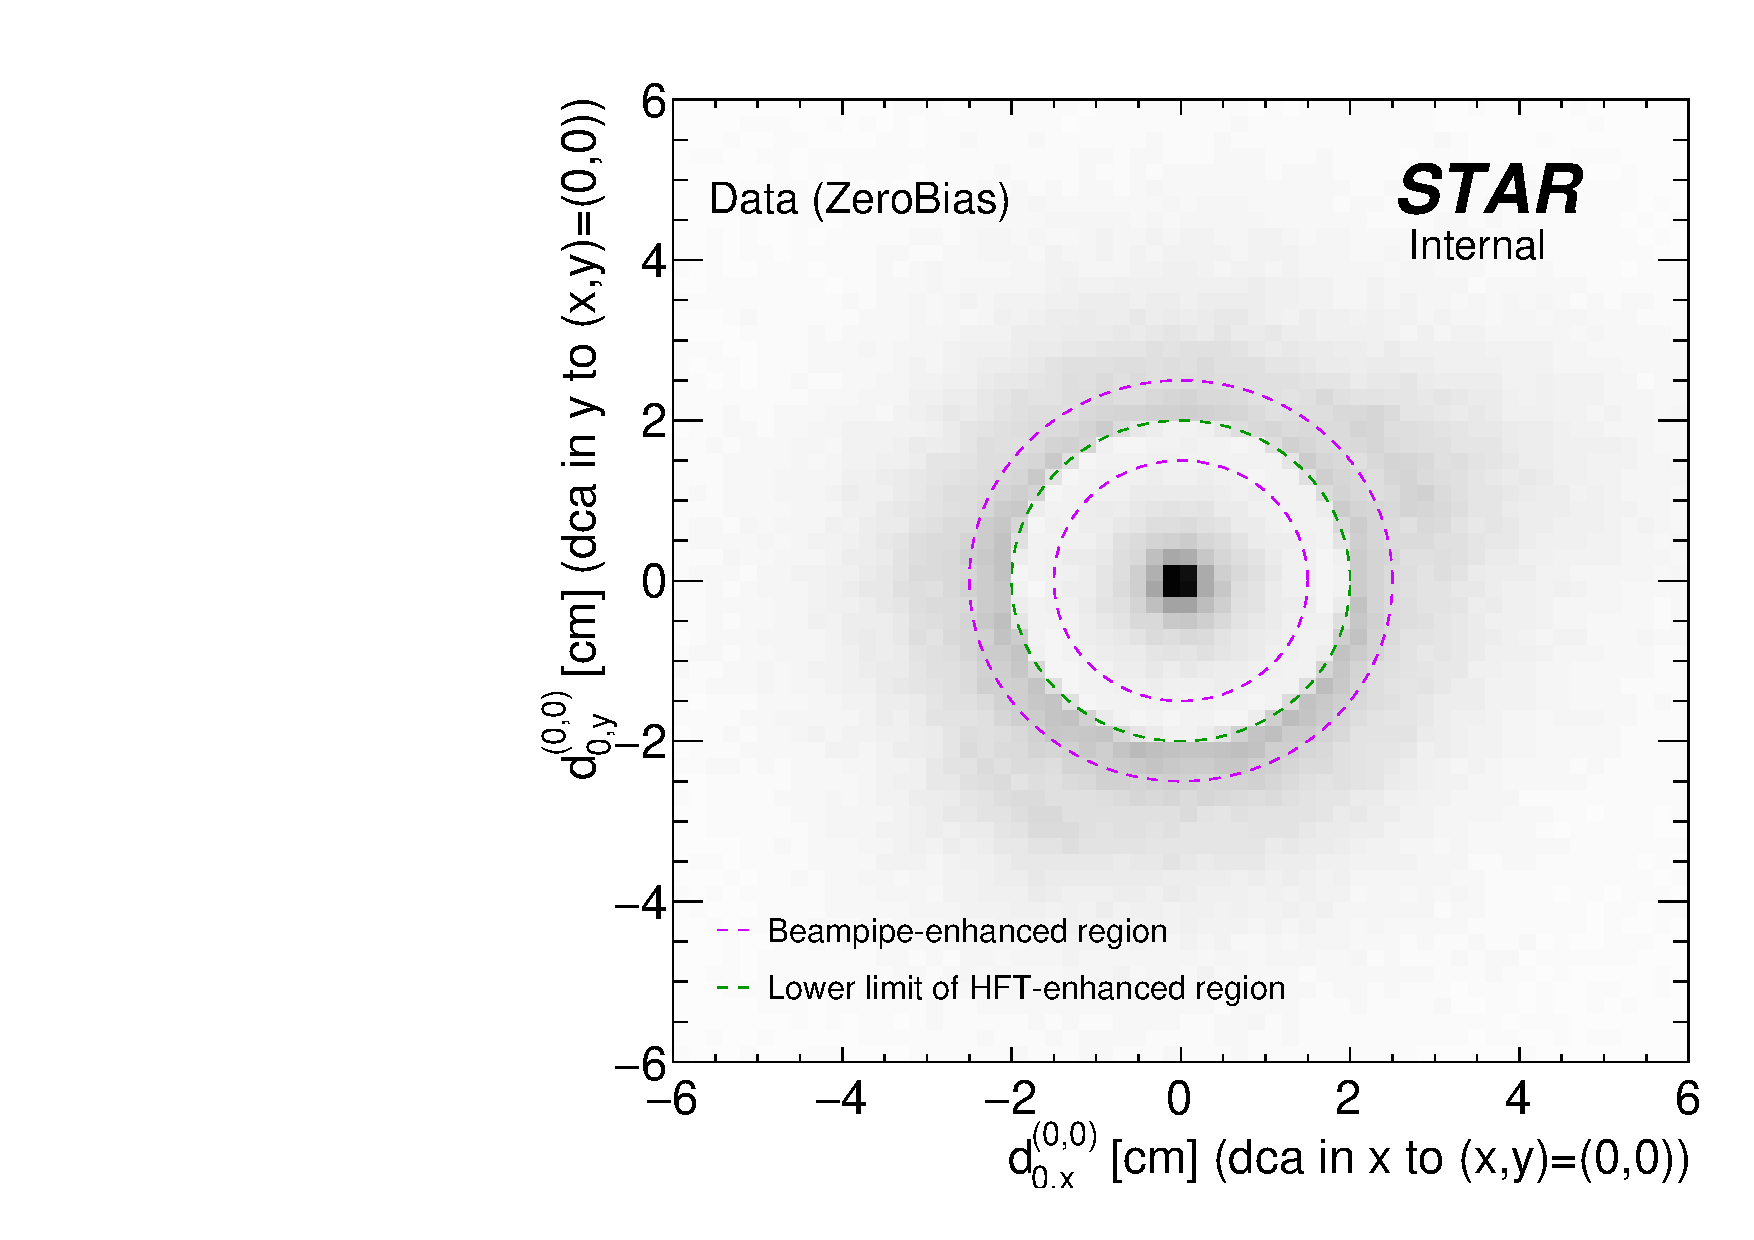
\includegraphics[width=\linewidth,page=1]{graphics/deadMaterial/D0yVsD0xGlobalTofTrks_DataVsMC.pdf}}
  \end{subfigure}\\
  \begin{subfigure}[b]{\linewidth}\addtocounter{subfigure}{1}
                \subcaptionbox{\label{fig:D0GlobalTofTrks_DataVsMC}}{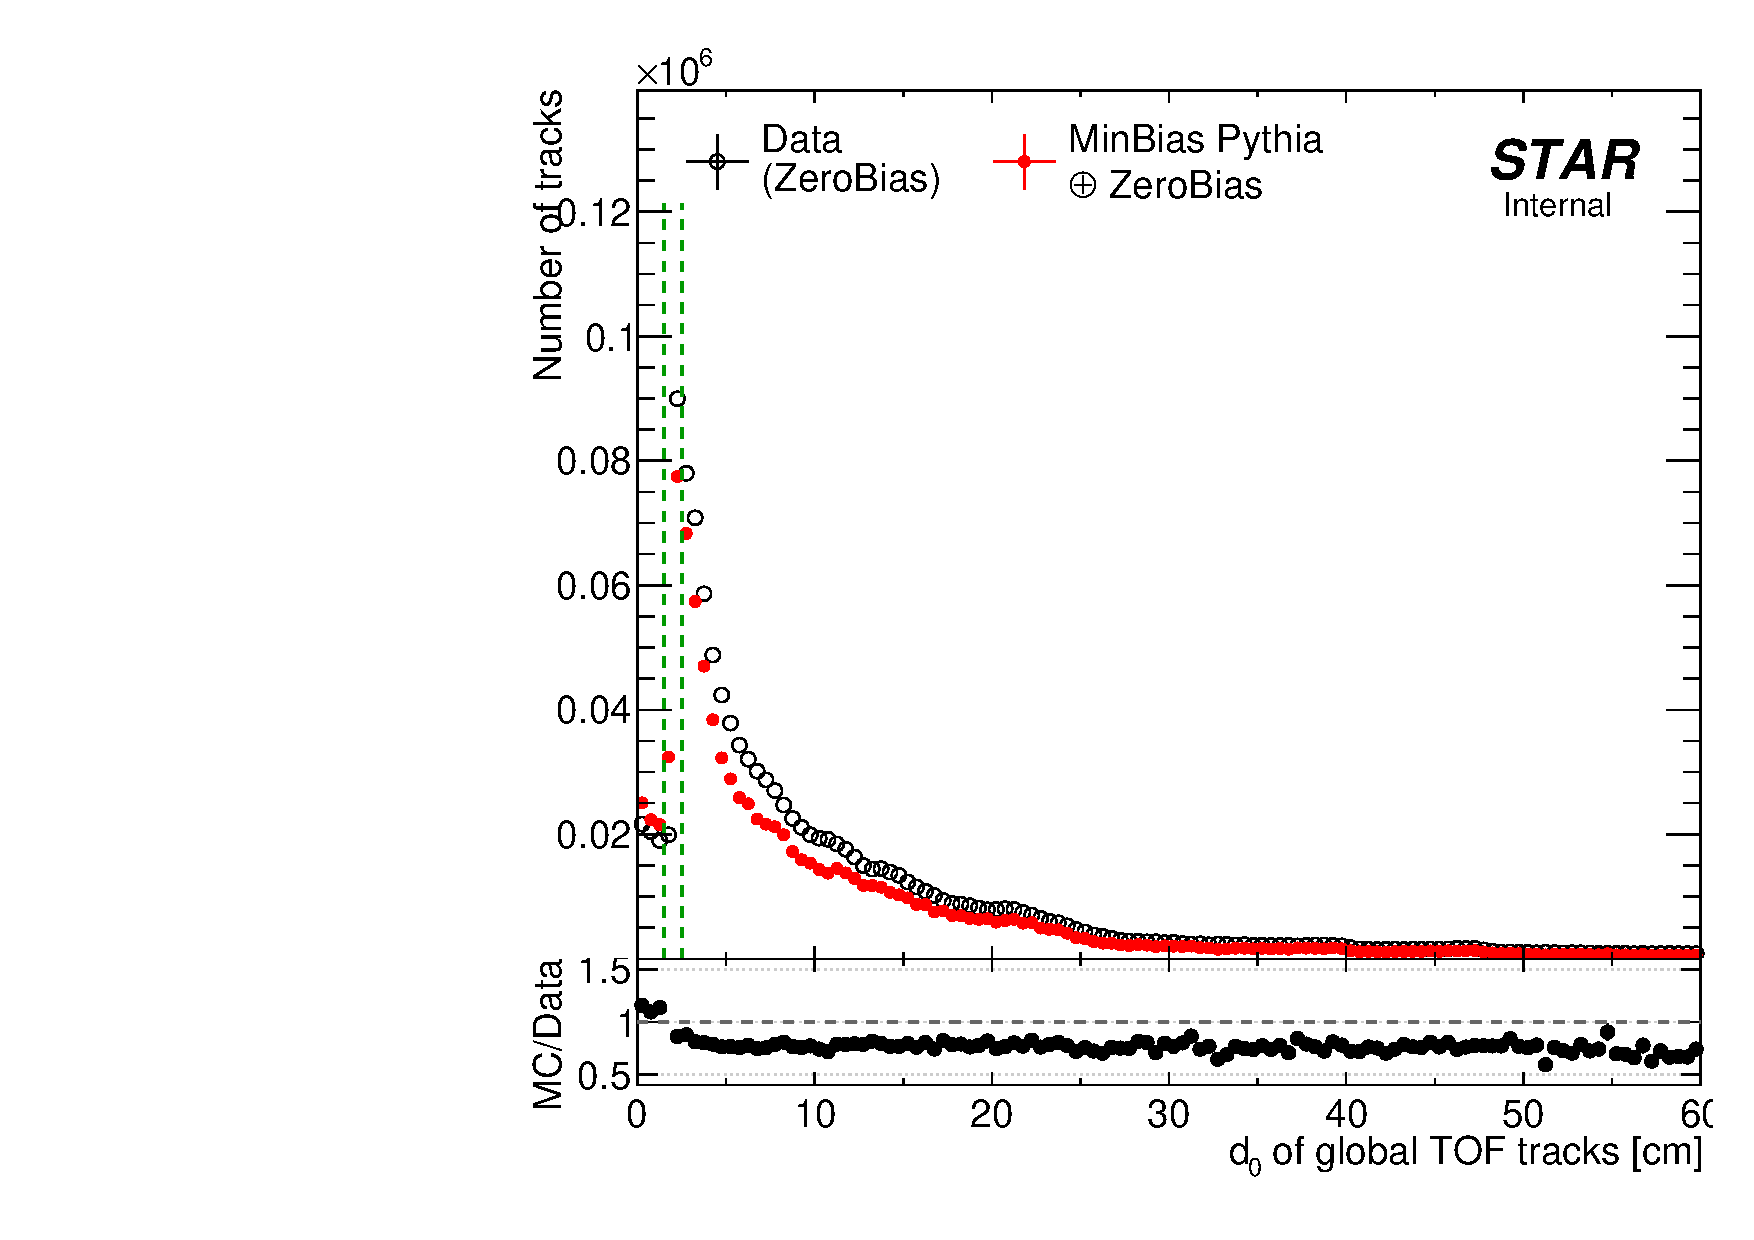
\includegraphics[width=\linewidth]{graphics/deadMaterial/D0GlobalTofTrks_DataVsMC.pdf}}
  \end{subfigure}
}%
\quad\quad%
\parbox{0.4725\textwidth}{
  \centering
  \begin{subfigure}[b]{\linewidth}\addtocounter{subfigure}{-2}
                \subcaptionbox{\label{fig:D0yVsD0xGlobalTofTrks_MC}}{\includegraphics[width=\linewidth,page=2]{graphics/deadMaterial/D0yVsD0xGlobalTofTrks_DataVsMC.pdf}}
  \end{subfigure}\\
  \begin{minipage}[t][1.042\linewidth][t]{\linewidth}\vspace{10pt}
    \caption[Comparison of $d_{0}^{(0,0)}$ distribution of global TPC tracks matched with TOF in zero-bias data and embedded MC (minimum-bias).]{Two-dimensional $d_{0}^{(0,0)}$ distribution of global TPC tracks matched with TOF in zero-bias data (\ref{fig:D0yVsD0xGlobalTofTrks_Data}) and embedded minimum-bias MC (\ref{fig:D0yVsD0xGlobalTofTrks_MC}), and comparison of their radial projection in wider range of $d_{0}^{(0,0)}$ (\ref{fig:D0GlobalTofTrks_DataVsMC}). Red dashed lines and arrow indicate limit of $d_{0}^{(0,0)}$ of tracks accepted for the secondary vertex analyses (limit equals 2~cm). In all subfigures there are only entries from global tracks not associated with the primary tracks. Even with relatively low pointing resolution of the TPC tracks ($\sim$1~cm) one can recongnize structures which can be atrributed the beampipe starting at $d_{0}^{(0,0)}=2$~cm, and HFT elements at about 8~cm, 11~cm, 14~cm and 22~cm.}\label{fig:deadMatDataVsMC2}
  \end{minipage}
}\vspace{-30pt}%
\end{figure}
%---------------------------

As a next step the TPC tracks were selected for the search and reconstruction of secondary vertices. The requirements were as follows:\vspace{-5pt}
\begin{enumerate}
  \item Global TPC tracks matched with TOF not associated with any primary TPC track,\vspace{-8pt}
  \item $|\eta|<0.7$,~~~~~~~~$p_{T}>0.2~\text{GeV}/c$,~~~~~~~~$N_{\textrm{hits}}^{\textrm{fit}}\geq25$,~~~~~~~~$N_{\textrm{hits}}^{\textrm{dE/dx}}\geq15$,~~~~~~~~$N_{\textrm{hits}}^{\textrm{fit}}/N_{\textrm{hits}}^{\textrm{poss}}\geq0.52$,\vspace{-8pt}
  \item Distance of closest approach to the STAR $z$-axis $(x, y)=(0, 0)$, $d_{0}^{(0,0)}$, larger than inner radius of the beampipe: $d_{0}^{(0,0)}>2$~cm.
\end{enumerate}%
These cuts were intended to select in-time TPC tracks with high chance of being a product of secondary interaction of primary particle with the detector material. The higher limit of accepted $d_{0}^{(0,0)}$ was set in analysis, the less background was found in the secondary vertex distribution for a price of limited access to secondary vertices of low radial distance from STAR $z$-axis. Cut of 2~cm was found a good compromise. In Fig.~\ref{fig:deadMatDataVsMC2} we present comparison of $d_{0}^{(0,0)}$ distribution of selected global TOF-matched TPC tracks in the data and embedded MC (without cut on $d_{0}^{(0,0)}$). To some extent this distribution reflects the material density (secondary vertex density) in the radial direction, therefore we present it with the MC distribution normalized to the same total number of primary tracks as in the data. Number of secondary vertices is proportional to the number of primary particles, so we use such normalization to allow direct comparison of the distributions:
\begin{equation}\label{eq:mcNormDeadMat}
\text{MC normalization factor}=\frac{\langle N_{\text{trks/evt}}^{\text{DATA}}\rangle \times N_{\text{evts}}^{\text{DATA}}}{ \langle N_{\text{trks/evt}}^{\text{MC}}\rangle \times N_{\text{evts}}^{\text{MC}} } = \frac{N_{\text{trks}}^{\text{DATA}}}{N_{\text{trks}}^{\text{MC}}}
\end{equation}%
Especially in Fig.~\ref{fig:D0GlobalTofTrks_DataVsMC} one can find structures/peaks that might be attributed to subdetectors (PXL, IST, SST) of the HFT. Notable is different yield of histograms which could indicate different amount of simulated dead material with respect to real conditions. The reason of this inconsistency was found in imperfect simulation of the pointing resolution of the TPC tracks - because the resolution is higher in the simulation, more true primary tracks is reconstructed as primary tracks hence less such tracks is accepted in the global track selection (comparing to data). This effect is accounted later in the background subtraction procedure.

After secondary track candidates were selected, the described algorithm for secondary vertex reconstruction was used:\\[-20pt]%
%---------------------------
\begin{wrapfigure}{o}{0.465\textwidth}\vspace{-\baselineskip}%
  \centering%
  ~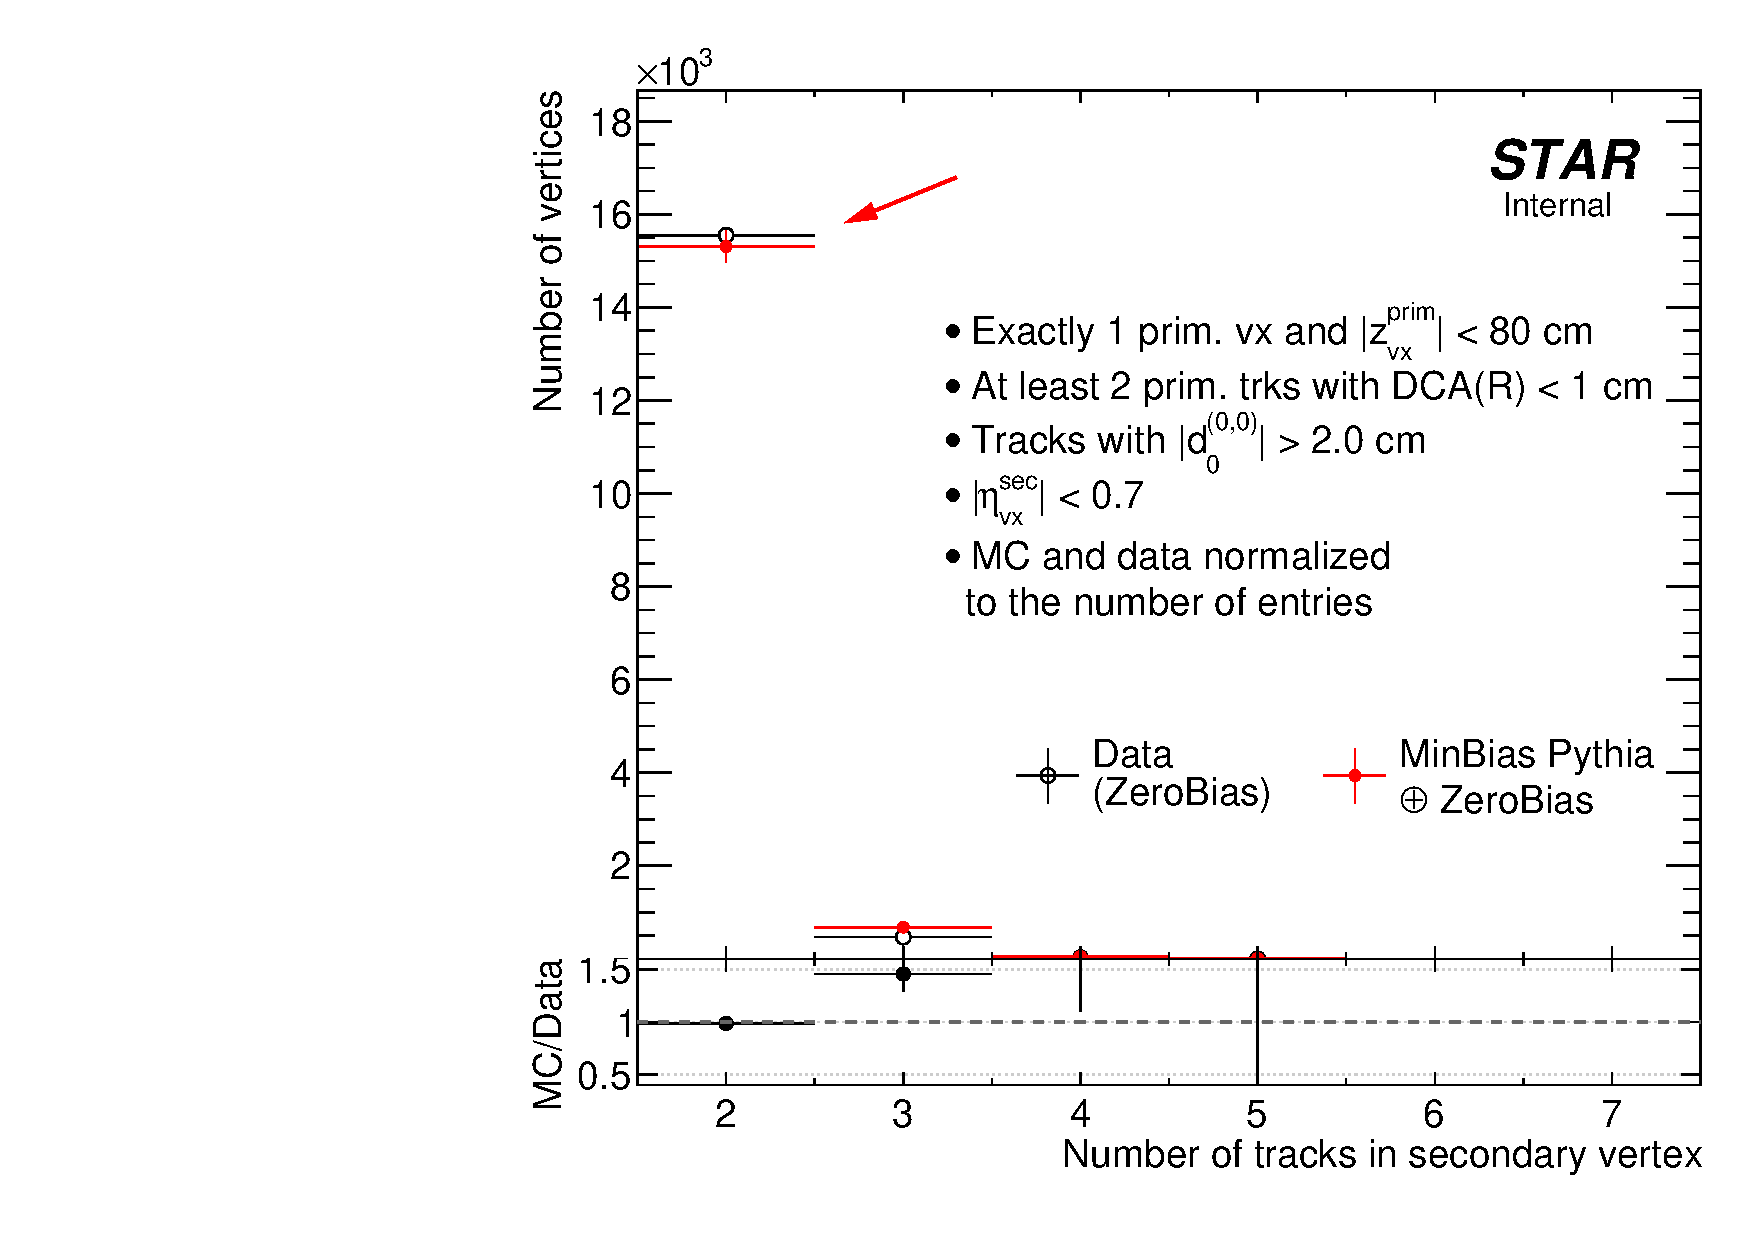
\includegraphics[width=0.465\textwidth]{graphics/deadMaterial/NTracksInVertex_DataVsMC.pdf}%
  \caption[Multiplicity of tracks in reconstructed secondary vertices.]{Multiplicity of tracks in reconstructed secondary vertices. Red arrow points to bin with vertices used in final comparisons of vertex position distribution.}\label{fig:nTrksInSecVx}\vspace{-30pt}%
\end{wrapfigure}%
%---------------------------
\vspace{-8pt}\begin{enumerate}
    \item Loop over all pairs of secondary track candidates, store pairs whose DCA is less than 0.5~cm (nearby tracks passing a proximity cut),\vspace{-8pt}
    \item Link pairs of nearby tracks into sets of tracks connected by the common nearby tracks,\vspace{-8pt}
    \item Loop over all sets defined in 2., in each set loop over all pairs from given set, reject worst-matching tracks (these with largest DCA to others) until all pairs of tracks have DCA less than 0.5~cm,\vspace{-8pt}
    \item Based on number of tracks in secondary vertex, total charge, specific energy loss, $dE/dx$, cosine of the opening angle of two tracks $cos(\theta)$ and invariant mass of two tracks $m_{\text{inv}}$ determine if the vertex is from resonance decay or photoconversion (see Ref.~\cite{deadMatSlides}); if none of the two then assume hadronic vertex,\vspace{-8pt}
    \item Calculate the vertex position as the average DCA point of all track pairs in the vertex.
   \end{enumerate}%
As a result secondary vertices were reconstructed, whose multiplicity distribution is depicted in Fig.~\ref{fig:nTrksInSecVx}.%
%---------------------------
\begin{wrapfigure}{l}{0.265\textwidth}\vspace*{-5pt}
  \centering
  ~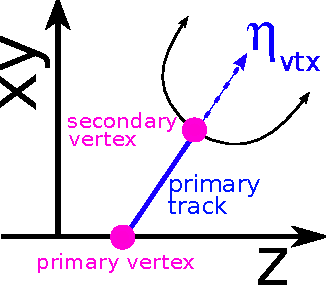
\includegraphics[width=0.265\textwidth]{graphics/deadMaterial/etaVxCut2.pdf}\vspace*{-5pt}
  \caption[$\eta_{\text{vtx}}$ definition (sketch).]{$\eta_{\text{vtx}}$ definition (sketch).}%
   \label{fig:etaVxCut} \vspace*{-9pt}
\end{wrapfigure}%\paragraph{}
%---------------------------
Analysis was continued only with vertices of multiplicity equal 2. The first reason was that most of vertices consist of just a pair of tracks. Another reason was the background subtraction method developed only for vertices made of two tracks. In addition to this, only vertices representing primary particles in the pseudorapidity range $-0.7 < \eta < 0.7$ were analyzed. To enable such selection a variable $\eta_{\text{vtx}}$ was defined, as shown in Fig.~\ref{fig:etaVxCut}.


Raw distributions of $R_{\text{vtx}}^{\text{secondary}}$ and $z_{\text{vtx}}^{\text{secondary}}$ are shown in Fig.~\ref{fig:RVertex_DataVsMC} and Fig.~\ref{fig:ZVertex_DataVsMC}, respectively. In $R_{\text{vtx}}^{\text{secondary}}$ spectrum one can find peaks in the regions where the HFT subdetectors are placed. Peaks seem to lie on top of a tail whose origin has been identified with the secondary vertices made of pairs containing true primary tracks which were not associated with any primary vertex and unfortunately passed selection of global tracks for the secondary vertex reconstruction. Without this backgroud subtracted, the ratio of MC to data varies mostly between 0.5 and 0.7. For this reason a method of estimation of the backgroud was invented, as described in the next paragraph.


%---------------------------
\begin{figure}[ht]
\centering
\parbox{0.4725\textwidth}{
  \centering
  \begin{subfigure}[b]{\linewidth}
                \subcaptionbox{\label{fig:RVertex_DataVsMC}}{\includegraphics[width=\linewidth,page=3]{graphics/deadMaterial/RVertex_DataVsMC.pdf}\vspace{-5pt}}
  \end{subfigure}
}%
\quad\quad%
\parbox{0.4725\textwidth}{
  \centering
  \begin{subfigure}[b]{\linewidth}
                \subcaptionbox{\label{fig:ZVertex_DataVsMC}}{\includegraphics[width=\linewidth,page=3]{graphics/deadMaterial/ZVertex_DataVsMC.pdf}\vspace{-5pt}}
  \end{subfigure}
}\vspace{-5pt}%
\caption[Comparison of raw $R_{\text{vtx}}^{\text{secondary}}$ and $z_{\text{vtx}}^{\text{secondary}}$ distribution in the data and embedded MC.]%
{Comparison of raw $R_{\text{vtx}}^{\text{secondary}}$ (\ref{fig:RVertex_DataVsMC}) and $z_{\text{vtx}}^{\text{secondary}}$ (\ref{fig:ZVertex_DataVsMC}) distribution in the data (opened black circles) and embedded MC (filled red circles). Only vertices recognized as products of hadronic interactions are shown in the figure. Solid lines denote estimated backgroud content in the distribution of corresponding color.}\vspace{-10pt}\label{fig:RZVertexDataVsMC}%
\end{figure}
%---------------------------


%---------------------------
\begin{figure}[b!]\vspace{-2pt}%
\centering%
\begin{minipage}{.4725\textwidth}%
  \centering%\vspace{11pt}
  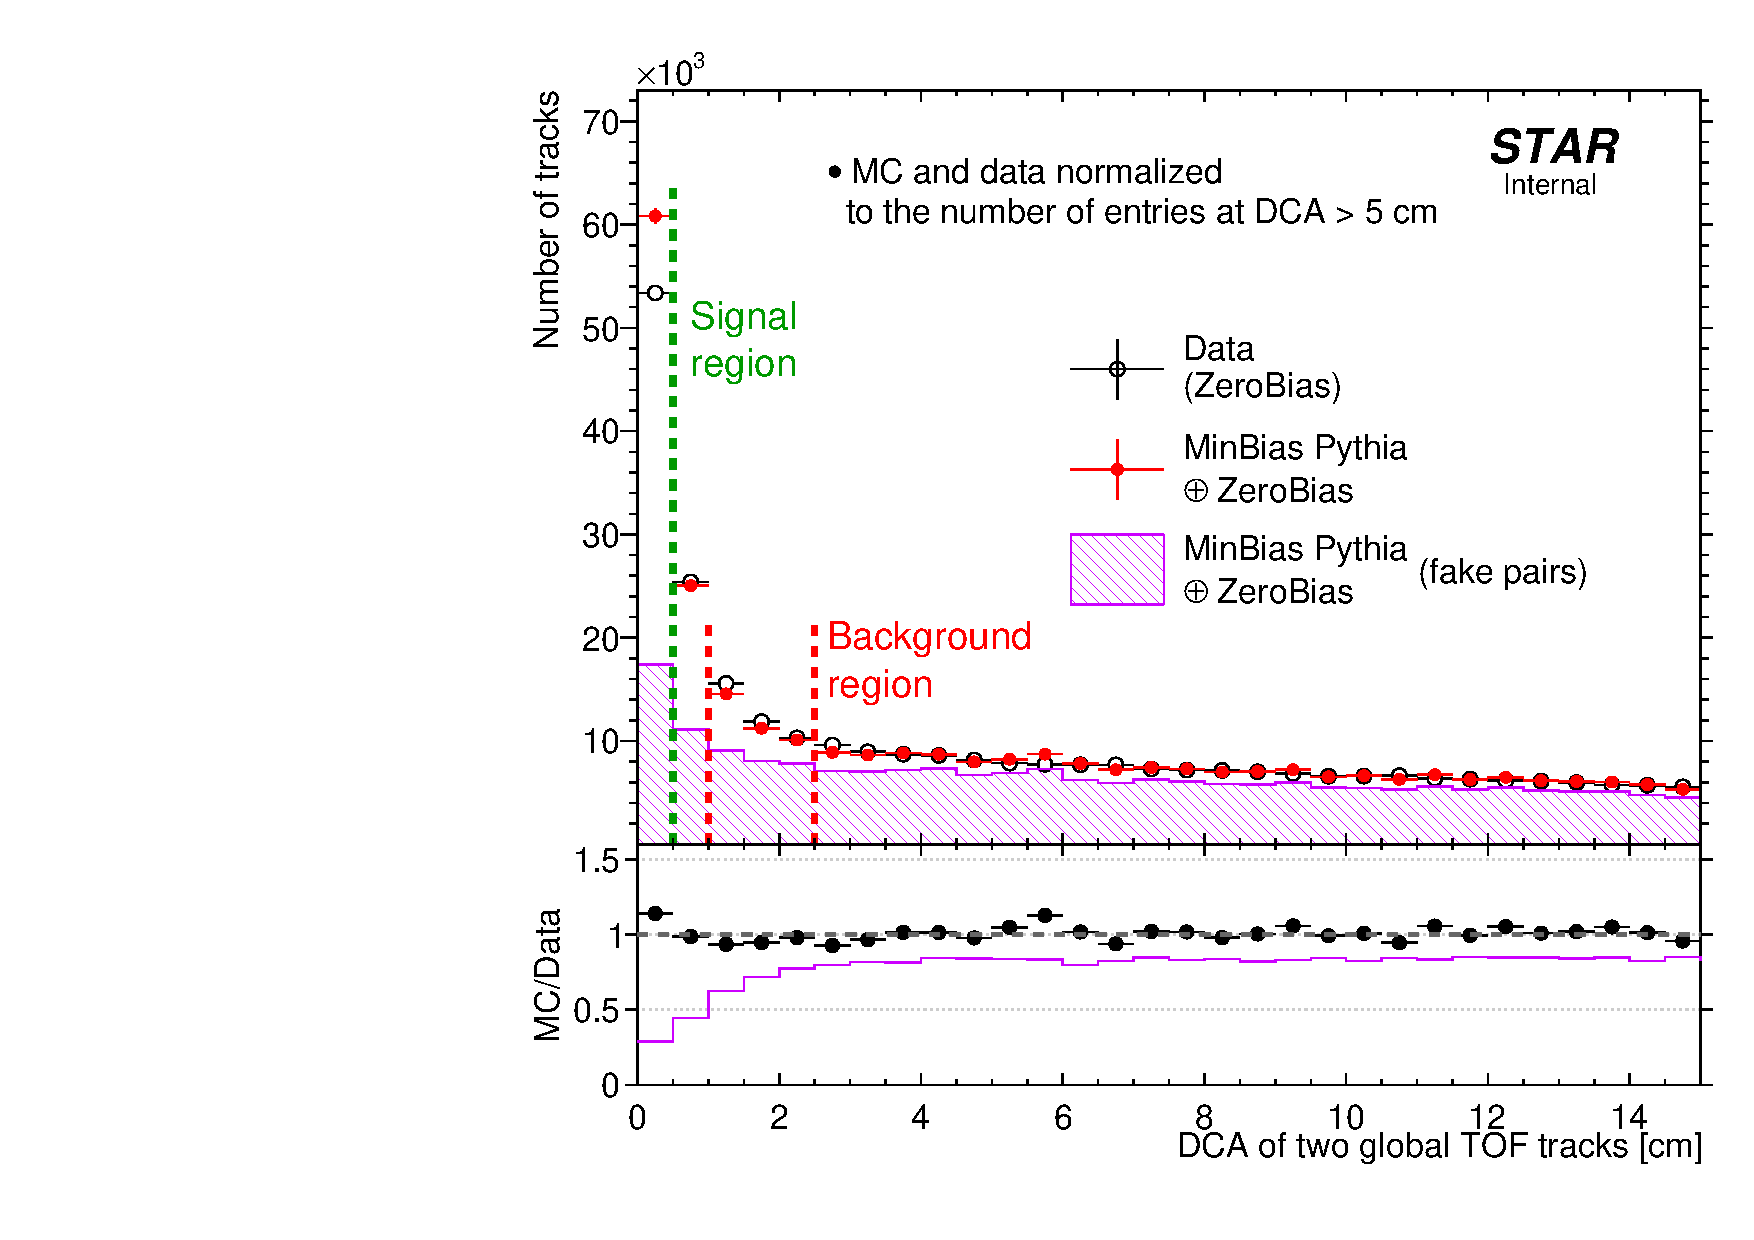
\includegraphics[width=\linewidth]{graphics/deadMaterial/DcaOfTwoGlobalTofTrksWithLargeD0_DataVsMC.pdf}\vspace{-5pt}%
  \caption[Comparison of DCA between all pairs of secondary track candidates selected for the secondary vertex reconstruction in the data and embedded MC.]%
  {Comparison of DCA between all pairs of secondary track candidates selected for the secondary vertex reconstruction  in the data and embedded MC. MC histogram is normalized to the data at $\text{DCA}>5$~cm. Violet hashed histogram depicts pairs contained in MC histogram and not originating from the same vertex. Solid violet line in the lower pad denotes ratio of violet and red histogram.\newline }\label{fig:DcaOfTwoGlobalTofTrksWithLargeD0_DataVsMC}
\end{minipage}%
\quad\quad%
\begin{minipage}{.4725\textwidth}%
  \centering%
  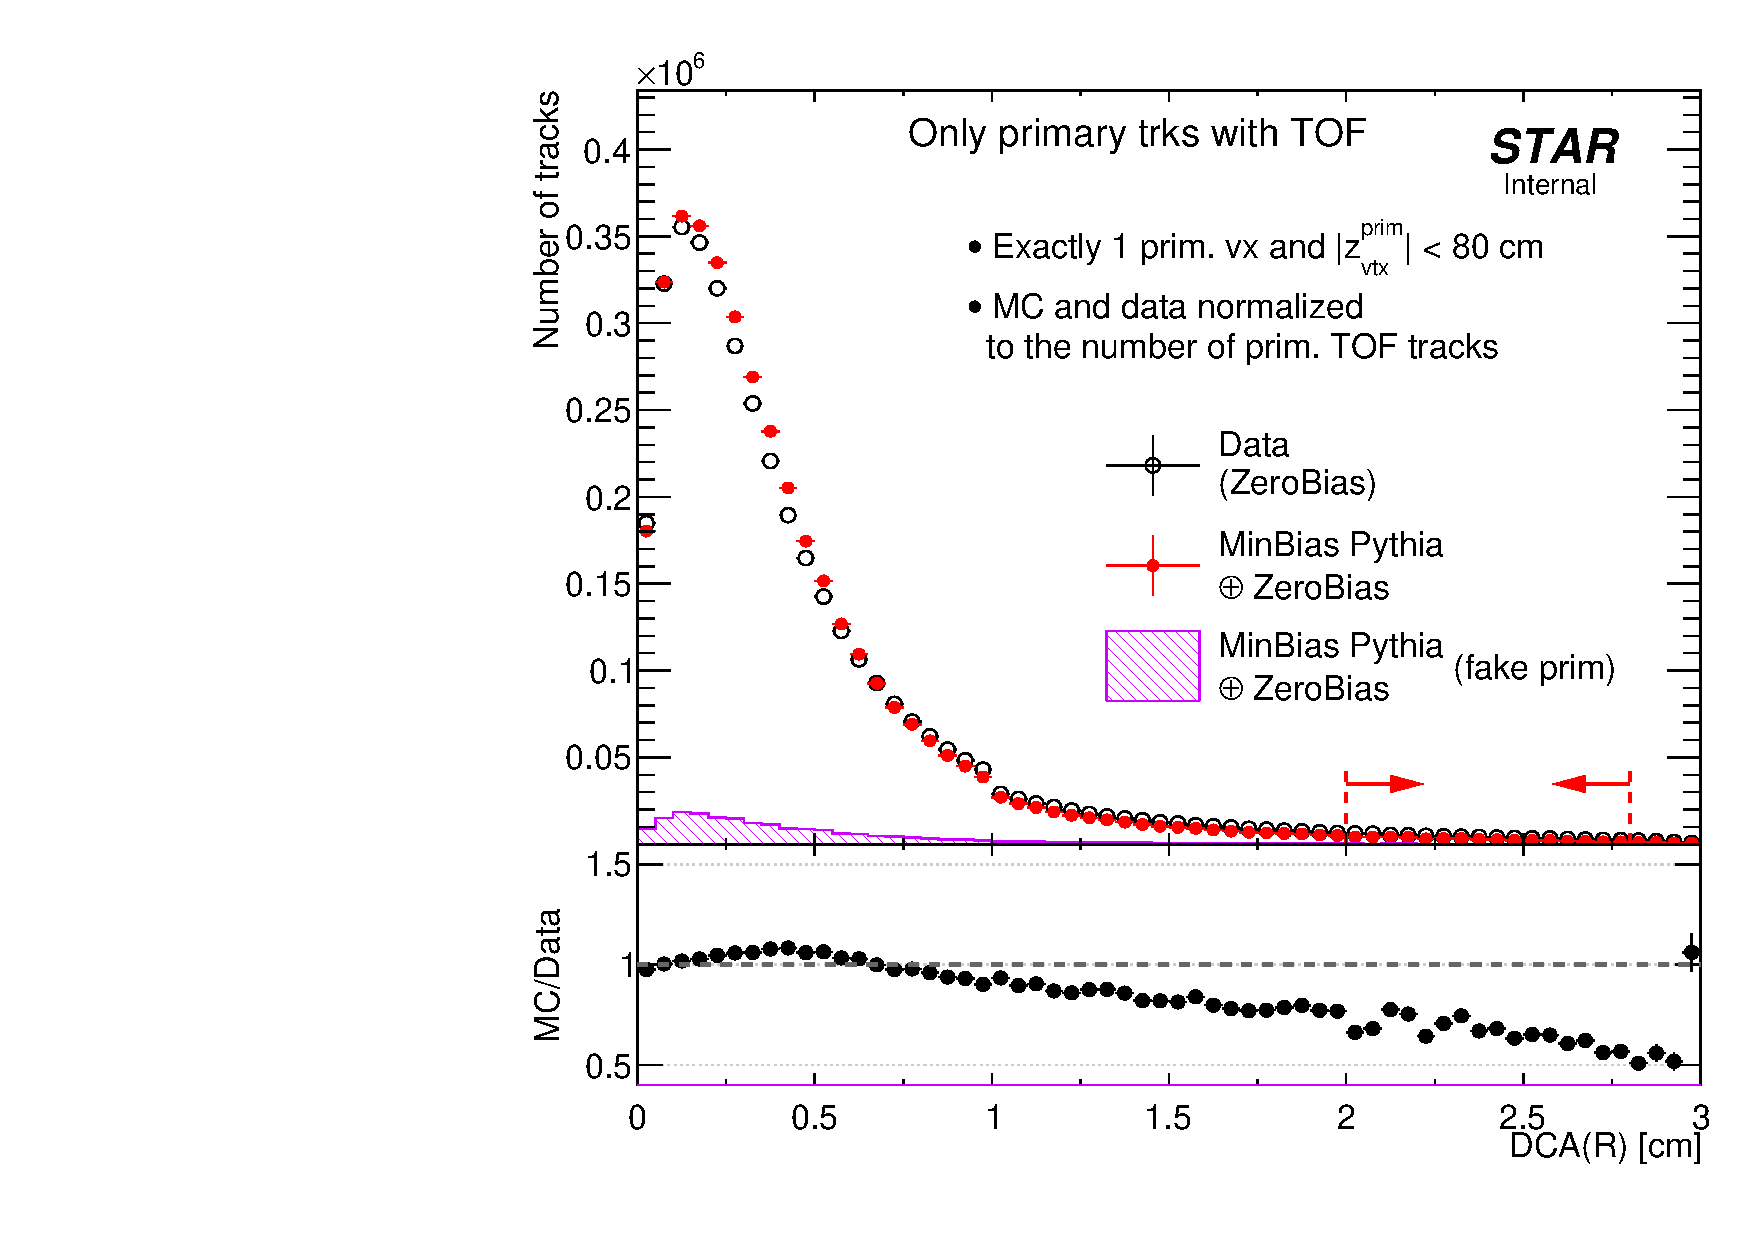
\includegraphics[width=\linewidth]{graphics/deadMaterial/DcaRPrimary_Tof_SelectedEvents_DataVsMC.pdf}\vspace*{-5pt}
  \caption[Comparison of radial DCA of all primary tracks matched with TOF and passing quality criteria in events selected for secondary vertex analysis, between the data and embedded MC.]
   {Comparison of radial DCA of all primary tracks matched with TOF and passing quality criteria in events selected for secondary vertex analysis, between the data and embedded MC. Violet hashed histogram represents tracks not matched to true-level particles. Red dashed lines and arrows limit region used to find normalization that compensates different backgroud yield in reconstructed secondary vertex distributions in data and embedded MC.}
   \label{fig:primaryDcaSelectedEvtsDataVsMC}%\vspace*{-29pt}
\end{minipage}%
\end{figure}%
%---------------------------

Background estimation makes use of different content of fake secondary vertices depending on the proximity cut used in the secondary vertex reconstruction. Figure~\ref{fig:DcaOfTwoGlobalTofTrksWithLargeD0_DataVsMC} shows the percentage of backgroud (fake pairs) distributed over the distance of closest approach between two tracks. A comment needs to be made that the agreement of the shape of the tails in data and MC distributions was achieved only after the adjustment of the TPC resoltion in MC, as described in Sec.~\ref{chap:tpcTrackPointingRes}. This agreement allows to believe in proper description of the data by MC in terms of backgroud distribution over DCA of two global tracks, which is used in the backgroud estimation.

It agrees with intuition that the most optimal cut to select pairs from the secondary vertices is as low as about 0.5~cm, however one can select sample with slightly different ratio of signal to background if the proximity cut is changed to accept tracks of DCA within some higher limits. In Fig.~\ref{fig:DcaOfTwoGlobalTofTrksWithLargeD0_DataVsMC} the nominal proximity cut is marked with the green line (signal region), while the modified proximity cut is marked with red lines (backgroud region). With such two versions of cuts used in vertexing the two independent distributions of secondary vertices can be obtained: one with the standard proximity cut - $\mathcal{H}_{1}$, the other with modified proximity cut, in our case $1.0~\text{cm}<\text{DCA}<2.5~\text{cm}$ - $\mathcal{H}_{2}$. Limits in modified proximity cut were set to such values in order to ensure enough statistics as well as provide satisfactory resolution of secondary vertex position calculated as a middle point between DCA points on helices associated with the tracks. One can note that the content of histograms can be described by the set of equations given below:
   \begin{empheq}[left=\empheqlbrace]{align}
     \mathcal{H}_{1} &= (1-B)\times\text{signal} + B\times\text{backgroud},\label{eq:h1} \\
     \mathcal{H}_{2} &= (1-B')\times\text{signal} + B'\times\text{backgroud},\label{eq:h2}
   \end{empheq}%
in which parameters $B$ and $B'$ denote the backgroud fraction in the distribution resultant from analysis utilizing nominal and modified proximity cut, respectively. The solution to set of Eqs.~\eqref{eq:h1},~\eqref{eq:h2} is the following:
   \begin{empheq}[left=\empheqlbrace]{align}
     \text{signal} &= \frac{B'\times \mathcal{H}_{1} - B\times \mathcal{H}_{2}}{B'-B}\label{eq:signal} \\
     \text{backgroud} &= \frac{(1-B)\times \mathcal{H}_{2} - (1-B')\times \mathcal{H}_{1}}{B'-B}\label{eq:bkgd}
   \end{empheq}%
An important remark here is that the backgroud fraction extracted from the ratio of violet and red histograms in Fig.~\ref{fig:DcaOfTwoGlobalTofTrksWithLargeD0_DataVsMC} can be used directly in Eqs.~\eqref{eq:h1}-\eqref{eq:bkgd} only for backgroud estimation in MC. In case of background estimation in data parameters $B$ and $B'$ have to be corrected for the leakage of true primary tracks to set of selected secondary track candidates, as it was decribed in one of preceding paragraphs. The correction factor $\kappa$ is extracted from the ratio of the radial DCA of the primary TPC tracks in events selected for the secondary vertex study. Histogram range selected for calculation of the ratio was set to $2.0~\text{cm}<\text{DCA}(R)<2.6~\text{cm}$, as this range coincides with the $d_{0}^{(0,0)}$ of global tracks accepted for the analysis. $\kappa$ calculated in this range equals 1.48. Variation of value of $\kappa$ with changed limits of DCA(R) selected for the ratio calculation do not influence significantly the final result. The correction is done by multiplying fraction $B$ and $B'$ by $\kappa$ only when estimating the backgroud in the data.

Backgroud determined with the described method is shown in Fig.~\ref{fig:deadMatDataVsMC} with the solid lines colored according to corresponding markers. This backgroud was subtracted and final, background-free distributions of the secondary vertex positions in the transverse and longitudinal direction are presented in Fig.~\ref{fig:RZVertexDataVsMC_BkgdSubtr}. Most releveant region - the HFT detector extending between $\sim$2~cm and $\sim$30~cm is satisfactorily well described by MC. Also, the inner wall of the TPC at $\sim$48~cm well matches between data and MC.



%---------------------------
\begin{figure}[hb]
\centering
\parbox{0.4725\textwidth}{
  \centering
  \begin{subfigure}[b]{\linewidth}
                \subcaptionbox{\label{fig:RVertex_DataVsMC_BkgdSubtr}}{\includegraphics[width=\linewidth,page=3]{graphics/deadMaterial/RVertex_BackgroudSubtracted_DataVsMC.pdf}}\vspace{-5pt}
  \end{subfigure}
}%
\quad\quad%
\parbox{0.4725\textwidth}{
  \centering
  \begin{subfigure}[b]{\linewidth}
                \subcaptionbox{\label{fig:ZVertex_DataVsMC_BkgdSubtr}}{\includegraphics[width=\linewidth,page=3]{graphics/deadMaterial/ZVertex_BackgroudSubtracted_DataVsMC.pdf}}\vspace{-5pt}
  \end{subfigure}
}%
\caption[Comparison of background-subtracted $R_{\text{vtx}}^{\text{secondary}}$ and $z_{\text{vtx}}^{\text{secondary}}$ distribution in the data and embedded MC.]%
    {Comparison of background-subtracted $R_{\text{vtx}}^{\text{secondary}}$ (\ref{fig:RVertex_DataVsMC_BkgdSubtr}) and $z_{\text{vtx}}^{\text{secondary}}$ (\ref{fig:ZVertex_DataVsMC_BkgdSubtr}) distribution in the data (opened black circles) and embedded MC (filled red circles). Only vertices recognized as products of hadronic interactions are shown in the figure.}\label{fig:RZVertexDataVsMC_BkgdSubtr}%
\end{figure}
%---------------------------